
\begin{figure}
\centering
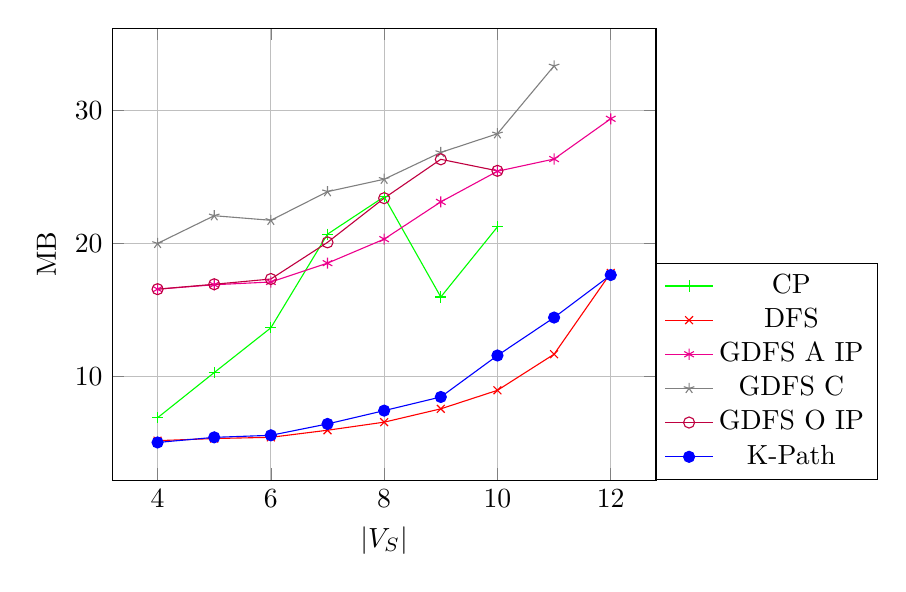
\begin{tikzpicture}
    \begin{axis}[
        xlabel=$|V_S|$,
        ylabel=MB,
        legend style={at={(1,0)},anchor=south west},
        width=0.7\textwidth,
		%y tick label style={/pgf/number format/sci},
        ymajorgrids,
        xmajorgrids,		
    ]

%    \node[] at (axis cs: 9,1.1) {Awaiting test results (CAES server)};

\addplot[
        mark=+,
        green,
    ] plot coordinates {
        (4,6.91822272)
        (5,10.31398616)
        (6,13.67548056)
        (7,20.71611176)
        (8,23.52690448)
        (9,15.993532618556701)
        (10,21.259674322580643)
%        (11,16.5165112)
%        (12,18.521343466666668)
%        (13,16.411888)
%        (14,16.529028)
};
    \addlegendentry{CP}
    
    \addplot[
        mark=x,
        red,
    ] plot coordinates {
        (4,5.19609856)
        (5,5.35496216)
        (6,5.4478832)
        (7,5.97976608)
        (8,6.58554064)
        (9,7.58865008)
        (10,8.97949888)
        (11,11.69218336)
        (12,17.800791342465754)
%        (13,9.0436)
%        (14,25.9406536)
%        (15,5.3708)
%        (16,5.372144)
};
    \addlegendentry{DFS}

    \addplot[
        mark=asterisk,
        magenta,
    ] plot coordinates {
        (4,16.58171168)
        (5,16.9127544)
        (6,17.12123872)
        (7,18.53596096)
        (8,20.3423896)
        (9,23.14127072)
        (10,25.44388352)
        (11,26.36181755102041)
        (12,29.385635243243243)
%        (13,26.053012)
%        (14,21.1499024)
};
    \addlegendentry{GDFS A IP}
    
    \addplot[
        mark=star,
        gray,
    ] plot coordinates {
        (4,20.02119344)
        (5,22.10080816)
        (6,21.75724016)
        (7,23.91128176)
        (8,24.84235504)
        (9,26.85778328)
        (10,28.26183368)
        (11,33.36203552)
%        (12,32.659569714285716)
%        (13,29.430532)
%        (14,35.4538864)
};
    \addlegendentry{GDFS C}
    
    \addplot[
        mark=o,
        purple,
    ] plot coordinates {
        (4,16.58121152)
        (5,16.950362)
        (6,17.34425624)
        (7,20.09879472)
        (8,23.4200908)
        (9,26.33993632)
        (10,25.47518344)
%        (11,22.3310536)
%        (12,23.083658153846155)
%        (13,16.653136)
%        (14,16.644884)
};
    \addlegendentry{GDFS O IP}
    
    \addplot[
        mark=*,
        blue,
    ] plot coordinates {
        (4,5.05997632)
        (5,5.44454632)
        (6,5.59800472)
        (7,6.4527912)
        (8,7.45263664)
        (9,8.47941568)
        (10,11.59705448)
        (11,14.44848288)
        (12,17.643857014084507)
%        (13,7.988368)
%        (14,9.271233142857144)
%        (15,5.362408)
%        (16,5.3676)
};
    \addlegendentry{K-Path}
	
    \end{axis}
    \end{tikzpicture}
    \caption{Space usage of the algorithm with each path iterator. $|V_T|=1\frac{1}{2}*|V_S|$, source vertices are ordered by GreatestConstrainedFirst, target vertices are ordered by degree, contraction is disabled, ``refusing longer paths" and no pruning is used.}
    \label{fig:spaceusage-pathiterators}

\end{figure}
